% Capítulo 5: while (testa antes) e do-while (testa depois).
\documentclass[border=4pt]{standalone}
\usepackage[utf8]{inputenc}
\usepackage[T1]{fontenc}
% Estilo comum dos fluxogramas e diagramas de blocos.
\usepackage{tikz}
\usetikzlibrary{arrows.meta, positioning, calc, shapes.geometric, shapes.misc}
\definecolor{navy}{RGB}{23,45,80}
\definecolor{laranja}{RGB}{250,110,29}
\definecolor{cinzalogo}{RGB}{107,114,126}
\definecolor{azul}{RGB}{205,222,247}
\tikzset{
  base/.style={draw=navy, line width=0.9pt, font=\sffamily\small, align=center, inner sep=4pt},
  terminal/.style={base, rounded rectangle, fill=laranja!45, draw=laranja, minimum width=20mm, minimum height=7mm},
  processo/.style={base, rectangle, fill=laranja!12, minimum width=28mm, minimum height=8mm},
  decisao/.style={base, diamond, aspect=2.2, fill=azul, inner sep=1pt, minimum width=30mm},
  es/.style={base, trapezium, trapezium left angle=72, trapezium right angle=108,
             fill=white, minimum width=26mm, minimum height=8mm, trapezium stretches body},
  fluxo/.style={-{Stealth[length=2.2mm]}, navy, line width=0.9pt},
  rotulo/.style={font=\sffamily\small\bfseries, text=navy},
  legenda/.style={font=\sffamily\scriptsize, text=cinzalogo},
  resposta/.style={font=\sffamily\scriptsize\bfseries, text=navy},
}

\tikzset{linha/.style={navy, line width=0.9pt}}
\begin{document}
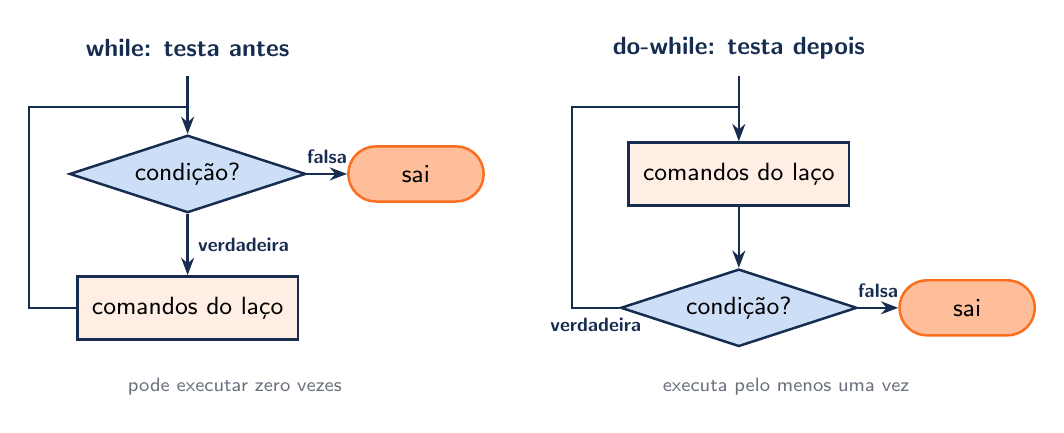
\begin{tikzpicture}
  % while
  \node[rotulo] at (0, 1.3) {while: testa antes};
  \node[decisao] (d1) at (0, -0.3) {condição?};
  \node[processo] (b1) at (0, -2.0) {comandos do laço};
  \node[terminal] (s1) at (2.9, -0.3) {sai};
  \coordinate (m1) at (0, 0.55);
  \draw[fluxo] (0, 0.95) -- (d1.north);
  \draw[fluxo] (d1) -- node[resposta, right] {verdadeira} (b1);
  \draw[linha] (b1.west) -- ++(-0.6, 0) |- (m1);
  \draw[fluxo] (d1) -- node[resposta, above] {falsa} (s1);
  \node[legenda, align=center] at (0.6, -3.0) {pode executar zero vezes};

  % do-while
  \node[rotulo] at (7, 1.3) {do-while: testa depois};
  \node[processo] (b2) at (7, -0.3) {comandos do laço};
  \node[decisao] (d2) at (7, -2.0) {condição?};
  \node[terminal] (s2) at (9.9, -2.0) {sai};
  \coordinate (m2) at (7, 0.55);
  \draw[fluxo] (7, 0.95) -- (b2.north);
  \draw[fluxo] (b2) -- (d2);
  \draw[linha] (d2.west) -- ++(-0.6, 0) node[resposta, below, pos=0.5] {verdadeira} |- (m2);
  \draw[fluxo] (d2) -- node[resposta, above] {falsa} (s2);
  \node[legenda, align=center] at (7.6, -3.0) {executa pelo menos uma vez};
\end{tikzpicture}
\end{document}
